\section{Einleitung}

\subsection{Motivation neuronaler Netze}
Heutzutage findet man in nahezu allen Bereichen des Lebens Programme vor, sei es in Zahnbürsten, Autos oder in Robotern am Fließband. Mithilfe von Programmen sollen also sich wiederholende Aufgaben vereinfacht oder automatisiert werden. Dafür werden die Programme mit prozedurale oder objektorientierte Methoden entwickelt. Bevor mit der Programmierung angefangen werden kann, muss zuerst ein Modell des Problems entworfen werden. Bei einfachen Anwendungen, wie zum Beispiel einer Zahnbürste ist es recht einfach. Möchte man allerdings ein Modell für eine Mustererkennung realisieren, stößt man mit herkömmlichen Methoden der Programmierung schnell an die Grenzen des machbaren. An dieser Stelle kommen neuronale Netze ins Spiel, die die Vorteile des menschlichen Denkens und Verhaltens emulieren sollen. Denn das menschliche Denken und Verhalten unterscheidet sich sehr stark von dem einer Maschine. Eine Maschine kann in der Regel nicht kreativ sein, Lösungen interpolieren, aus Fehlern lernen und phantasievoll sein.

Bei der klassischen Programmierung spricht man auch von einer symbolischen Informationsverarbeitung. Alle Schritte sind dem Programmierer bewusst und er kann genau sagen, wie sich sein Programm verhalten wird. Vorausgesetzt er hat vorab ein präzises Modell erarbeitet. Dem Gegenüber steht die Programmierung mit neuronalen Netzen. Bei neuronalen Netzen spricht man von einer sub-symbolischen Informationsverarbeitung. Der Programmierer des neuronalen Netzwerkes kann trotz eines genauen Modells nicht 100\% sicher sagen, wie sich das neuronale Netzwerk am Anfang verhalten wird. Erst wenn das neuronale Netzwerk konfiguriert wurde, ist es möglich genaueres Verhalten des neuronalen Netzes abzuschätzen. Die sub-symbolische Programmierung ist immer dann einzusetzen, wenn es schwer möglich ist die 'Realwelt' perfekt als Modell abzubilden. 

\begin{quote}
    Die Grundidee der sub-symbolischen Informationsverarbeitung ist das Auflösen der Symbole zur Beschreibung der Anwendungswelt in Mikrostrukturen auf der Basis primitiver Verarbeitungseinheiten (simulierter Neuronen). \cite[S. 9]{Kratzer1991} 
\end{quote}

Um besser zu verstehen, wie Nervenzellen (Neuronen) funktionieren, handelt der nächste Abschnitt über das menschliche Nervensystem.

\subsection{Das menschliche Nervensystem}
Das menschliche Gehirn besteht aus etwa 86 Milliarden Nervenzellen, auch Neuronen genannt, die zum Zentralnervensystem miteinander verschaltet sind (im folgendem Nervensystem).\cite{dasgehirn.info} Nervenzellen im Gehirn sind hochspezialisierte Zellen, die sich im Gegensatz zu einfacheren Zellen nicht teilbar sind. Das bedeutet, dass sich das Nervensystem nicht über Zellteilung regenerieren kann. Allerdings schafft es das Gehirn durch die Verknüpfung anderer Nervenzellen den Defekt teilweise oder komplett auszugleichen. Jede Nervenzelle kann mit bis zu 10.000 anderen Nervenzellen in Verbindung stehen.\cite{gehirnlernen.de} 

Jede Nervenzelle ist im Grundaufbau gleich, kann aber unterschiedliche Formen und Größen haben. Das liegt unter anderem daran, dass sich Nervenzellen weiter spezialisieren.\cite{gehirnlernen.de} So können die einen Nervenzellen für motorische und die anderen für sensorische Aufgaben bestimmt sein. Dadurch erreichen Nervenzellen unterschiedliche Geschwindigkeiten, wie sie Informationen an andere Nervenzellen weitergeben.\cite{dasgehirn.info} Der Informationsfluss ist dabei immer in die gleiche Richtung.\cite{gehirnlernen.de} In Abbildung \ref{fig:AufbauNeuron} ist der Aufbau einer Nervenzelle dargestellt.

\begin{figure}[hbt]
	\centering
	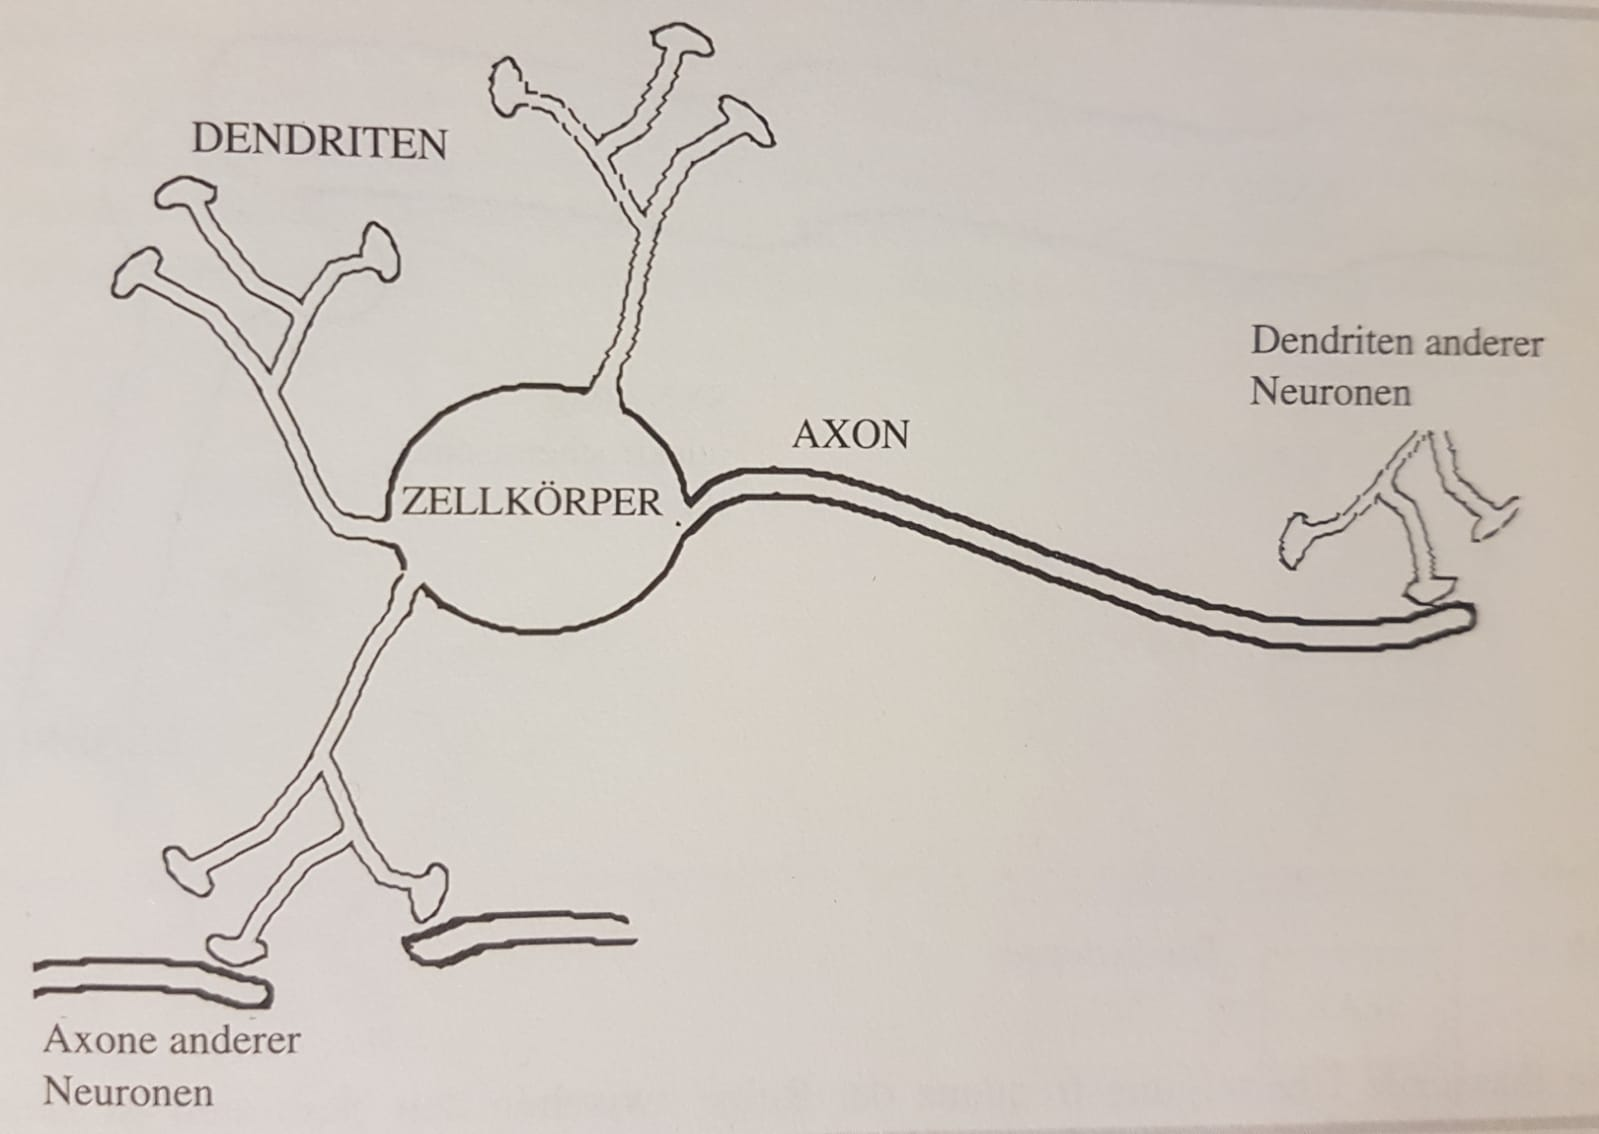
\includegraphics[width=0.9\linewidth]{./Bilder/Aufbau_Nervenzelle_Mazzetti}
	\caption{Aufbau Neuron \cite[S. 11]{Mazzetti1996}}
	\label{fig:AufbauNeuron}
\end{figure}

Der hier stark vereinfachte Aufbau einer Nervenzelle besteht aus dem Zellkörper, den Dendriten, dem Axon und den Synapsen. Die Synapsen liegen jeweils am Ende der Dendriten und des Axons. Der Zellkörper bildet die zentrale Einheit einer Nervenzelle und erhält seine Informationen über die Dendriten. Die Dendriten sind baumartig verzweigt und mit anderen Nervenzellen über Synapsen verbunden. Der Zellkörper bildet eine Summation über die Signale der vielen verschieden Dendriten. Dabei kann jedes Dendrit eine erregende oder hemmende Wirkung auf den Zellkörper haben. Bei ausreichender Stärke leitet der Zellkörper das Signal weiter. Wenn eine Erregungsweiterleitung stattfindet, wird das Signal über das Axon und Synapsen an die nächste Nervenzelle weitergeleitet. Ein Axon hat einen Durchmesser von 0,002 - 0,01 Millimetern und kann bis zu einem Meter lang sein.\cite{gehirnlernen.de} Umso dicker ein Axon ist, desto schneller findet auch die Weiterleitung statt. Jede Nervenzelle kann nur über ihre Synapsen mit anderen Nervenzellen kommunizieren. Dafür hat jede Nervenzelle bis zu 10.000, in manchen Extremfälle sogar mehr als 100.000 Synapsen.\cite{dasgehirn.info} Synapsen kommunizieren untereinander mit chemischen oder elektrischen Signalen. Wobei elektrische in chemische und chemische in elektrische Signale umgewandelt werden. In der Regel kommunizieren Synapsen über chemische Signale. Der Grund dafür ist, dass Synapsen meisten keinen direkten Kontakt zueinander haben, sondern ein kleiner Abstand von 20 bis 50 Nanometern bleibt.\cite{dasgehirn.info} Bei elektrischen Synapsen ist der Abstand so nah, dass über eine kleine Brücke (gap junction) kommuniziert wird. Dabei kann das Signal schneller weitergeleitet werden.\cite{gehirnlernen.de}

Das Nervensystem ist ein großes Netz aus sehr vielen Nervenzellen, die unterschiedlich stark miteinander verbunden sind und unterschiedlich schnell Signale weiterleiten. Wenn eine Nervenzelle ein Signal auslöst, weil eine gewisse Schwelle überschritten wurde spricht man auch davon, dass das Aktionspotenzial erreicht wurde. Das Aktionspotenzial kann nur erreicht werden, wenn vorher genügend vorgeschaltete Nervenzellen ein Signal gesendet haben. Der Anfang einer Verkettung von Nervenzellen kann zum Beispiel über sehen, schmecken, spüren oder ähnliches stattfinden. Wird ein Aktionspotenzial in den dafür verantwortlichen Nervenzellen erreicht, werden sie wieder Signale an andere Nervenzellen senden. Am Ende kann das Signal bei Nervenzellen ankommen, die für eine Bewegung verantwortlich sind, wie zum Beispiel eine Gehbewegung. Das ist ein sehr stark vereinfachtes Beispiel und soll nur dazu dienen die Mechanismen eines Nervensystems zu verstehen.

\begin{figure}[hbt]
	\centering
	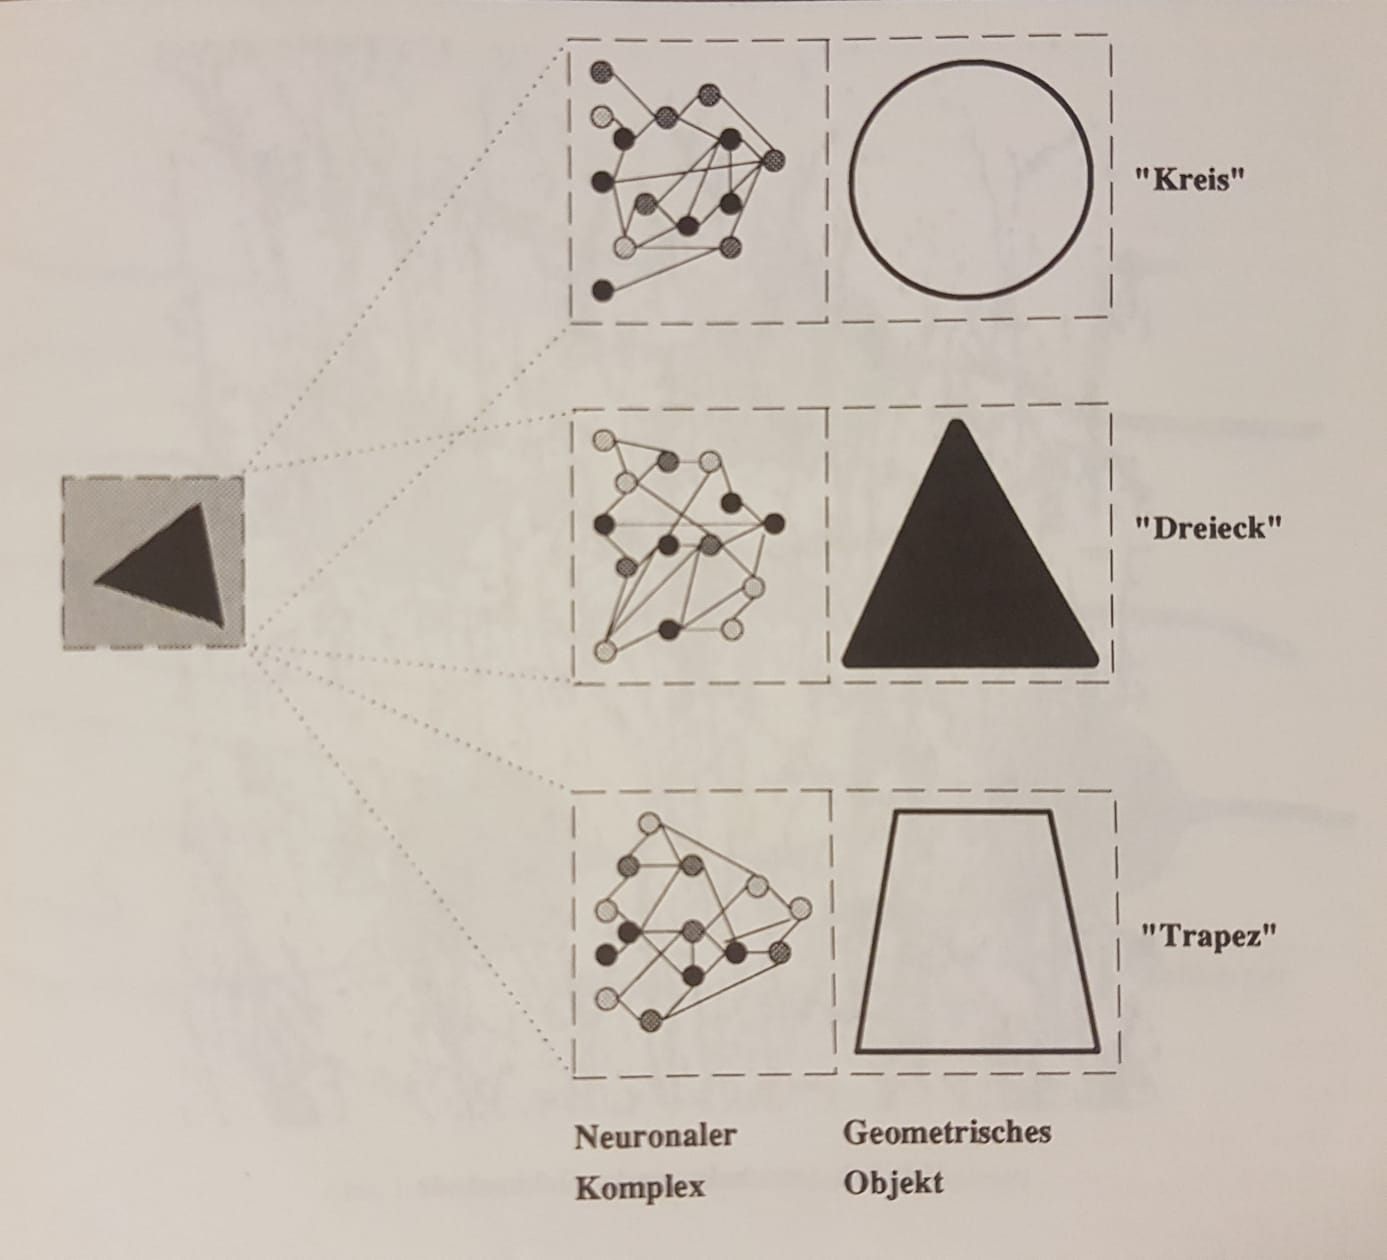
\includegraphics[width=0.9\linewidth]{./Bilder/VerarbeitungVisuellerEindruck-Kratzer}
	\caption{Vearbeitung eines visuellen Eindrucks \cite[S. 9]{Kratzer1991}}
	\label{fig:visuelleVerarbeitung}
\end{figure}

In Abbildung \ref{fig:visuelleVerarbeitung} ist zu sehen, wie ein visueller Eindruck in einem neuronalen Netzwerk verarbeitet wird. Im neuronale Netzwerk werden bei verschiedenen visuellen Eindrücken verschiedene Neuronen unterschiedlich stark stimuliert. Umso mehr sich Objekte voneinander unterscheiden, desto mehr wird sich auch das neuronale Netzwerk in der Stimulation der einzelnen Neuronen unterscheiden. Dabei gibt es nicht nur zwei Stufen der Unterscheidung, sondern mehrere. Kennt man die Stimulationen der einzelnen Neuronen auf verschiedene geometrische Referenz-Objekte, wie eines 'Kreis', 'Dreieck' oder 'Trapez' kann man neue unbekannte geometrische Objekte mit bekannten vergleichen und eine Aussage darüber treffen, um was es sich für ein Objekt handelt. Die Entscheidung ist dabei mit Wahrscheinlichkeiten verbunden. Ist die Übereinstimmung mit einem Referenz-Objekt sehr hoch, wird es auch möglich sein eine gute Aussagekraft über das unbekannte Objekt zu erhalten. Umso mehr sich ein unbekanntes Objekt von den Referenz-Objekten unterscheidet, desto geringer wird auch die Aussagekraft über das unbekannte Objekt sein.

\subsection{Neuronale Netze und ihre Bedeutung - Quelle angeben}
Um besser zu verstehen, wie das menschliche Gehirn funktioniert wurden von Biologen, Neurophysiologen und Kognitionswissenschaftler neuronale Verarbeitungsmodelle entwickelt. Bei den entwickelten Verarbeitungsmodelle ist darauf zu achten, dass sie sehr stark vereinfacht sind. Sie sollen viel mehr genutzt werden, um Theorien zu untertermauern. Die Verarbeitungsmodelle umfassen eine Vielzahl von Annahmen der menschlichen Gehirnstruktur, die nicht eindeutig belegt sind.

\begin{quote}
    Neuronale Netzwerke sind Modelle der Gehirnfunktion. Sie versuchen, in Struktur und Funktionsweise Gehirnzellkomplexe nachzubilden und dadruch eine tragfähige Simulation komplexer menschlicher Denkvorgänge zu erzielen. \cite[S. 12]{Kratzer1991} 
\end{quote}

Am menschlichen Gehirn sind nicht nur die kreativen und phantasievollen Fähigkeiten erstaunlich. Auch die Fähigkeit etwas neues zu lernen und neue Lösungen für Probleme zu finden. Wenn Teile des menschlichen Gehirns beschädigt werden, wie zum Beispiel durch einen Schlaganfall, schafft es das menschliche Gehirn die auftretenden neurologischen Ausfälle teilweise bzw. komplett zu regenerieren. All diese Vorteile können nicht mit einem herkömmlichen Programm nachgebildet werden und es Bedarf die Implementierung eines künstlichen neuronalen Netzwerks. Dabei müssen nicht alle Facetten des menschlichen Gehirns nachgebildet werden, sondern nur grundlegende Funktionen.

Ein Vorteil, die ein künstliches neuronales Netz übernehmen kann von einem menschlichen Gehirn sind unter anderem die Robustheit. Wenn bei einem hinreichend großem Netz ein Neuron ausfällt, dann können umliegende Neuronen die Aufgabe übernehmen, wenn man das neuronale Netzwerk neu anlernen würde. Aber auch bei nicht neu anlernen des Netzwerkes würde zwar die Qualität der Aussage schlechter werden, aber es könnten immer noch Aussagen getroffen werden. Dies gilt bei Aufgabenstellungen, die  assoziierenden, interpolierenden, klassifizierenden oder beurteilenden Charakter haben.

Ein zweiter Vorteil von künstlichen neuronalen Netzen in der modernen Mehrprozessor-Rechner-Architektur sind die Modellinhärenten Parallelisierungsmöglichkeiten. So können Neuronen zu bestimmten Gruppen zusammengefasst werden, ähnlich wie es auch im menschlichen Nervensystem realisiert wird, und sehr stark miteinander vernetzt sein. Jede Gruppe wird dann auf verschiedenen Prozessoren ausgeführt und nur notwendige Verbindungen über die Prozessoren hinaus verbunden. Das gilt natürlich nicht nur für Software-, sondern auch für Hardwareimplementierungen.

Ein dritter Vorteil von künstlichen neuronalen Netzen ist die Adaptivität, also die Fähigkeit etwas zu erlernen. Dafür gibt es für fast jedes Netzmodell Verfahren, die es dem Netzwerk erlauben sich selbst zu konfigurieren. Soll ein neuronales Netzwerk Muster erkennen, dann werden dem neuronalen Netzwerk vorab Beispiele für zu erkennende Muster gegeben und damit das Netzwerk konfiguriert. Man spricht davon auch von Trainingsbeispielen. Diese Trainingsbeispiele sollten möglichst reproduzierbar sein. Am Ende des Trainings soll das neuronale Netzwerk bisher unbekannte Muster durch Assoziation bzw. Interpolations erkennen.

Trotz dieser ganzen Vorteile künstlicher neuronaler Netze ist es nicht möglich zukünftig ohne die klassische Programmierung auszukommen. Für jede neue Anwendung muss immer eine Ein- und Ausgabecodierung vorliegen. Wie soll der Anwender am Ende sonst erkennen, wie das Ergebnis zu interpretieren ist. Bei den Ein- und Ausgaben handelt es sich um teils komplexe Transformationen. Neuronale Netzwerke bieten eine großen Einsatzbereich, sind aber nicht in der Lage die herkömmliche Programmierung komplett zu ersetzen. Es kommt vielmehr auf das Einsatzgebiet an, wo man mehr mit neuronalen Netzwerken, mit herkömmlichen Programmiermethodiken oder mit einer Kombination arbeitet.